\documentclass[11pt]{amsart}
\input{glyphtounicode}
\pdfgentounicode=1
\usepackage[T1]{fontenc}
\usepackage[utf8]{inputenc}
\usepackage{amsmath,amssymb,amsthm,mathtools}
\usepackage{array,booktabs,tabularx}
\usepackage{graphicx}
\usepackage{xcolor}
\usepackage{geometry}
\usepackage{enumitem}
\usepackage{hyperref}
\geometry{margin=1in}
\setlength{\emergencystretch}{3em}
\graphicspath{{../tree_stability_v4/figures/}}
\hypersetup{colorlinks=true,linkcolor=blue!45!black,citecolor=blue!45!black,urlcolor=blue!45!black,
  pdftitle={Source-Resolved Error Calculus for Projected Multilinear Computational Graphs},
  pdfauthor={Eliuth Chavero Jasso},
  pdfsubject={DAG provenance, higher-order source polynomials, and signed cancellation certificates},
  pdfkeywords={computational DAG, error provenance, source polynomial, cancellation certificate}}
\newtheorem{theorem}{Theorem}[section]
\newtheorem{proposition}[theorem]{Proposition}
\newtheorem{corollary}[theorem]{Corollary}
\theoremstyle{definition}
\newtheorem{definition}[theorem]{Definition}
\theoremstyle{remark}
\newtheorem{remark}[theorem]{Remark}
\newcommand{\norm}[1]{\lVert#1\rVert}
\newcommand{\op}{\mathrm{op}}
\newcommand{\cF}{\mathfrak F}
\newcommand{\cP}{\mathcal P}

\title[Source-resolved error calculus]{Source-Resolved Error Calculus for Projected Multilinear Computational Graphs}
\author{Eliuth Chavero Jasso}
\address{Independent Researcher, Apizaco, Tlaxcala, Mexico}
\thanks{Research manuscript. The results are finite and conditional on the stated algebraic and norm hypotheses. Novelty and independent human review remain pending.}
\date{8 August 2026 -- v5 research manuscript}

\begin{document}
\begin{abstract}
Recursive projection creates local closure residuals that can be propagated through trees and directed acyclic graphs. This paper consolidates a finite source-resolved calculus developed in the repository: scalar DAG majorants, first-order vector provenance, exact higher-order source polynomials with repeated-source multi-indices, and signed compositional aggregation. The central refinement is to combine coefficients by source and multi-index before taking norms, yielding certified inequalities $B_{\rm actual}\le B_{\rm signed}\le B_{\rm treewise}$ and strict cancellation witnesses. Associator, Jacobiator, and Filippov defects are treated as instances of one signed-expression engine; no identity is assumed to vanish. Approximate-law representation error and validated norm enclosures are recorded as separate certificate layers.\end{abstract}
\subjclass[2020]{15A69, 18M60, 65G50, 68N30}
\keywords{multilinear computational graph, DAG, error provenance, source polynomial, signed cancellation, validated certificate}
\maketitle

\section{Why a graph calculus?}

Tree certificates are safe but can overcount shared subcomputations. If one
source fans out and returns through multiple paths, a pathwise triangle bound
norms every route before remembering that the routes originated from the same
error. Signed identities introduce a second loss: independently bounding each
term destroys cancellation between bracketings or forest terms. The v4/v5
implementation addresses both losses while preserving the finite algebraic
semantics of recursive projection.

\section{Typed DAG model}

Let $G=(V,E)$ be a finite typed DAG with a designated output node. Each node
$v$ has a multilinear law $\mu_v$ and receives already computed values from
its predecessors. Let $F_v$ denote the ambient value and $R_v$ the recursively
projected value. The local difference is $D_v=F_v-R_v$. A local normal source
is labelled by $s$ and written $\varepsilon_s$; it may be a closure residual,
an approximate-law residual, or another explicitly registered source family.

For scalar nonnegative summaries, assume
\begin{equation}
 B_v\le\lambda_v+\sum_{u\to v}h_{v,u}B_u,
 \qquad \lambda_v,h_{v,u}\ge0.
 \label{eq:scalar}
\end{equation}

\begin{theorem}[Scalar DAG source certificate]
\label{thm:scalar}
Let $\widehat B_v$ be defined by equality in~\eqref{eq:scalar} in topological
order. Define $w_r=1$ at the output $r$ and, in reverse topological order,
\[
 w_u=\sum_{v:u\to v}h_{v,u}w_v.
\]
Then
\[
 B_r\le\widehat B_r=\sum_{u\in V}\lambda_u w_u.
\]
The calculation is $O(|V|+|E|)$ and does not enumerate paths.
\end{theorem}

The term $\lambda_u w_u$ is a source-resolved attribution. If the output
projection annihilates the root local residual, the root source is omitted
from the observable projected certificate.

\section{First-order source provenance}

At first order, the error at each node can be represented as
\begin{equation}
 D_v^{(1)}=\sum_s A_{v,s}\varepsilon_s.
 \label{eq:first-order}
\end{equation}
The operators $A_{v,s}$ are propagated in topological order. If a source
reaches the output over paths $\pi$, the source-aware operator is
\[
 A_{r,s}=\sum_{\pi:s\leadsto r}A_\pi.
\]
Thus
\[
 \norm{D_r^{(1)}}\le\sum_s\norm{A_{r,s}}\,\norm{\varepsilon_s}
 \le\sum_s\sum_{\pi:s\leadsto r}\norm{A_\pi}\,\norm{\varepsilon_s}.
\]

\begin{corollary}[Source refinement]
The first-order source-aware certificate is never larger than the pathwise
triangle certificate built from the same path operators. Strict improvement is
possible when routes from a shared source cancel.
\end{corollary}

\section{Exact nonlinear source polynomials}

Sets of sources are insufficient when the same source is used in two slots.
Let $\alpha=(\alpha_s)_{s\in\mathcal S}$ be a finite multi-index with total
order $|\alpha|=\sum_s\alpha_s$. Write $[\varepsilon^\alpha]$ for the
corresponding multilinear source monomial, including repeated occurrences.

\begin{definition}[Source polynomial]
The source polynomial at node $v$ is the finite formal expansion
\[
 \cP_v(\varepsilon)=
 \sum_{\alpha\ne0}A_{v,\alpha}[\varepsilon^\alpha],
 \qquad D_v=\cP_v(\varepsilon).
\]
\end{definition}

\begin{theorem}[Exact finite DAG provenance]
For a finite DAG of multilinear laws with finitely many labelled local
sources, the source polynomial at every node is obtained exactly by topological
recurrence. When a law receives source polynomials with multi-indices $\alpha$
and $\beta$ in different slots, the product term carries index $\alpha+\beta$.
Consequently a repeated source used in two slots produces a term with
$\alpha_s=2$. On a tree, the construction reduces to the ordinary child-error
subset expansion after forgetting global source labels.
\end{theorem}

The exact implementation is finite for finite declared DAGs. Truncation is
allowed only with an explicit tail envelope:
\[
 D_v=D_v^{(\le p)}+R_v^{(>p)},
 \qquad \norm{R_v^{(>p)}}\le\mathcal R_v^{(p)}.
\]
The repository tests $p=1,2,3$ and repeated-source, mixed-source, shared
subexpression, projected-root, real, and complex controls.

\section{Signed compositional expressions}

Let
\[
 \cF=\sum_{j=1}^m c_jT_j
\]
be a finite signed expression, where each $T_j$ has source coefficients
$A_{j,\alpha}$. Aggregate before taking norms:
\[
 A_{\cF,\alpha}=\sum_{j=1}^m c_jA_{j,\alpha}.
\]
For source amplitudes $t_s$, define
\[
 B_{\rm signed}=\sum_\alpha
 \norm{A_{\cF,\alpha}}\prod_s|t_s|^{\alpha_s},
\]
whereas treewise aggregation gives
\[
 B_{\rm treewise}=\sum_j|c_j|\sum_\alpha
 \norm{A_{j,\alpha}}\prod_s|t_s|^{\alpha_s}.
\]

\begin{theorem}[Signed source-polynomial refinement]
\label{thm:signed}
For every finite exact source polynomial and signed expression,
\[
 \boxed{B_{\rm actual}\le B_{\rm signed}\le B_{\rm treewise}}.
\]
The second inequality follows coefficient-wise from the triangle inequality.
It can be strict, including at orders $|\alpha|\ge2$ and for exact
cancellation.
\end{theorem}

\subsection{Associator, Jacobiator, and Filippov defects}

The associator is the signed expression $T_L-T_R$. The Jacobiator and
Filippov object are not assumed to vanish; the engine returns certificates for
the calculated defects under the registered conventions. This distinction is
essential: a small certified defect is not a proof that an arbitrary law
satisfies an identity.

For a truncation order $p$, the signed certificate is paired with the combined
remainder:
\[
 B_{\rm total}^{(p)}=B_{\rm signed}^{(\le p)}+
 B_{\rm remainder}^{(>p)}.
\]
Omitted terms are never cancelled by expectation.

\section{Approximate laws and norm enclosures}

If $\widetilde\mu_v$ approximates $\mu_v$, define
$\delta_v=\norm{\mu_v-\widetilde\mu_v}_\op$. Closure and representation
sources remain separately labelled. The output budget decomposes into closure,
representation, and interaction contributions, with nonlinear envelopes added
only when their Lipschitz hypotheses are explicit.

Norm estimation is likewise layered. An exact formula is preferred, followed
by validated interval enclosure, flattening/spectral bounds, CP-structure
bounds, and Frobenius fallback. Every output records lower bound, upper bound,
gap, method, and certification flag. An optimizer value alone is not called an
operator norm certificate.

\begin{figure}[p]
\centering
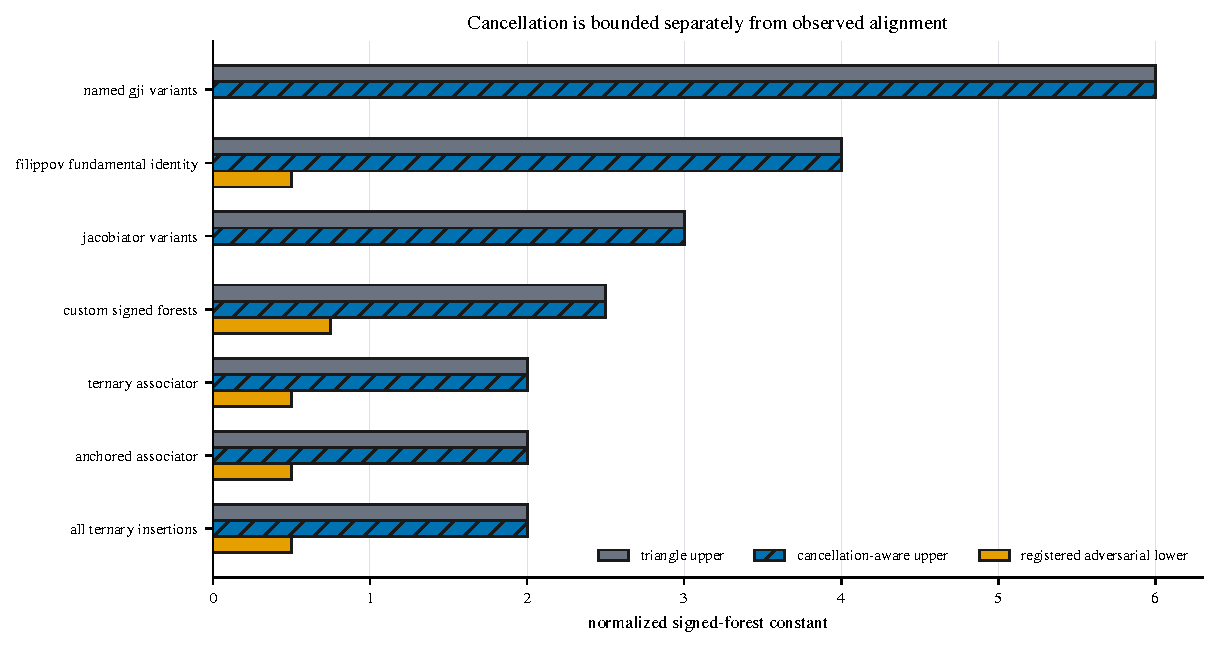
\includegraphics[width=.93\textwidth]{fig13_signed_polynomial_cancellation}
\caption{Signed source aggregation preserves cancellation before norm evaluation. Reused from the registered finite evidence package.}
\end{figure}

\begin{figure}[p]
\centering
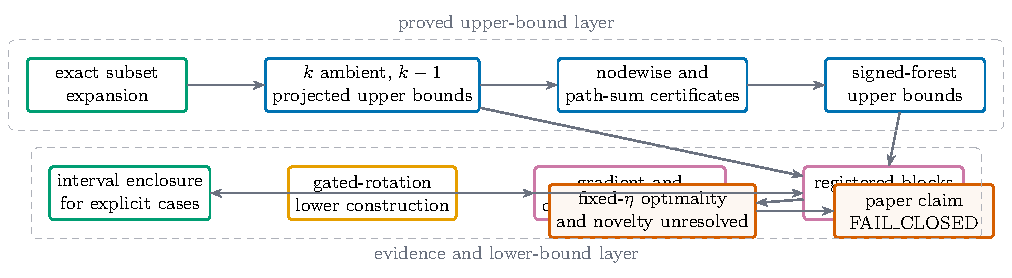
\includegraphics[width=.93\textwidth]{fig18_claim_evidence_dag}
\caption{Proof, certificate, construction, empirical search, and release authorization remain separate evidence layers.}
\end{figure}

\section{Status and open theorem problems}

The finite scalar DAG, first-order source, exact higher-order source
polynomial, signed expression, associator/Jacobiator/Filippov instantiations,
validated finite norm enclosures, and approximate-law budget interfaces are
implemented and tested in the v4/v5 research tracks. They are conditional on
their declared finite hypotheses. Remaining theorem-level questions include
global fixed-$\eta$ sharpness under repeated laws, dimension/rank reduction,
topology-aware constants, globally tight multilinear spectral norms, and
theorem-to-theorem novelty. The source package is therefore a closed finite
calculus, not a claim of universal optimality or publication approval.

\section{Conclusion}

The resulting framework tracks not only how much error reaches an output, but
which local sources generated it, how shared sources are reused, which higher
orders interact, and where signed cancellation survives. This source-resolved
calculus is the natural DAG extension of recursively projected multilinear
tree analysis.

\nocite{Yau2016,LodayVallette2012,Higham2002,KoldaBader2009,MooreKearfottCloud2009}
\bibliographystyle{amsplain}
\bibliography{references}
\end{document}
